% ============================================================
%  LAMPIRAN B – ARSITEKTUR KG REVIEW APP
%  Compile standalone:  pdflatex lampiran-b.tex
%  Compile as part of thesis: pdflatex main.tex
% ============================================================
\documentclass[main]{subfiles}
\usepackage{hyphenat}
\usepackage{iftex}

% ── Encoding, Language & Fonts ───────────────────────────────
\ifXeTeX
    \usepackage{polyglossia}
    \setmainlanguage{bahasai}
    \usepackage{fontspec}
    \setmainfont{TeX Gyre Termes}
    \setsansfont{TeX Gyre Heros}
    \setmonofont[Scale=0.88]{TeX Gyre Cursor}
\else
    \usepackage[utf8]{inputenc}
    \usepackage[T1]{fontenc}
    \usepackage[indonesian]{babel}
    \usepackage{mathptmx}
    \usepackage{helvet}
    \usepackage{courier}
\fi

% ── Page geometry (A4, UI thesis margins) ────────────────────
\usepackage[
  a4paper,
  top    = 2.54cm,
  bottom = 2.54cm,
  left   = 3.17cm,
  right  = 2.54cm
]{geometry}

% ── Line spacing & paragraph ─────────────────────────────────
\usepackage{setspace}
\onehalfspacing
\setlength{\parindent}{1.27cm}
\setlength{\parskip}{0pt}

% ── Microtype & justification ────────────────────────────────
\usepackage{microtype}
\sloppy

% ── Headings ─────────────────────────────────────────────────
\usepackage{titlesec}

\titleformat{\chapter}[block]
  {\centering\sffamily\bfseries\large}{}
  {0pt}{\MakeUppercase}
\titlespacing*{\chapter}{0pt}{0pt}{1.5em}

\titleformat{\section}
  {\sffamily\bfseries\normalsize}{\thesection}{1em}{}
\titlespacing*{\section}{0pt}{1.2em}{0.6em}

\titleformat{\subsection}
  {\sffamily\bfseries\normalsize}{\thesubsection}{1em}{}
\titlespacing*{\subsection}{0pt}{1em}{0.5em}

% ── Tables ───────────────────────────────────────────────────
\usepackage{longtable, booktabs, array, multirow}
\usepackage{calc}
\usepackage{tabularx}

% ── Graphics ─────────────────────────────────────────────────
\usepackage{graphicx}
\makeatletter
\def\maxwidth{\ifdim\Gin@nat@width>\linewidth\linewidth\else\Gin@nat@width\fi}
\makeatother
\setkeys{Gin}{width=\maxwidth,keepaspectratio}

% ── Lists ────────────────────────────────────────────────────
\usepackage{enumitem}

% ── Hyperlinks ───────────────────────────────────────────────
\usepackage[hidelinks]{hyperref}

% Bibliography setup is inherited from main.tex (biblatex + references.bib)
% when this file is compiled standalone via the subfiles class.

% ============================================================
\begin{document}

% When standalone: switch to appendix lettering and set the counter
% so \chapter{} renders as "LAMPIRAN B". When compiled inside main.tex,
% main.tex issues \appendix and advances the counter before \subfile.
\ifSubfilesClassLoaded{}{\appendix\setcounter{chapter}{1}}

\chapter{Arsitektur KG Review App}
\label{lamp:kg-review-app}

Lampiran ini merinci implementasi \textit{KG Review App}, yakni instrumen
validasi berbasis web yang digunakan pakar untuk meninjau \textit{triple}
hasil sistem (lihat Subbab~\ref{subsec:cara-pengumpulan}). Cakupan lampiran
meliputi \textit{tech stack}, diagram arsitektur, skema kunci penyimpanan
\textit{Redis}, serta tangkapan layar kedua antarmuka peninjauan (Fase~1 dan
Fase~2).

% ------------------------------------------------------------------
\section{Tech Stack}
\label{lamp:tech-stack}

Tabel~\ref{tab:tech-stack} merangkum komponen perangkat lunak yang
menyusun aplikasi beserta perannya.

\begin{table}[h]
  \centering
  \caption{\textit{Tech stack} KG Review App}
  \label{tab:tech-stack}
  \begin{tabularx}{\linewidth}{@{}l l X@{}}
    \toprule
    \textbf{Lapisan} & \textbf{Teknologi} & \textbf{Peran} \\
    \midrule
    Antarmuka      & Next.js (React) & Penyajian halaman peninjauan dan
                     interaksi pakar. \\
    Logika aplikasi & Next.js \textit{API routes} & Penanganan permintaan
                     anotasi dan agregasi keputusan. \\
    Penyimpanan    & Redis & Persistensi sesi peninjauan, antrean
                     \textit{triple}, dan rekam keputusan pakar. \\
    % TODO: tambahkan baris lain bila relevan (mis. autentikasi, deployment).
    \bottomrule
  \end{tabularx}
\end{table}

% ------------------------------------------------------------------
\section{Diagram Arsitektur}
\label{lamp:diagram-arsitektur}

Gambar~\ref{fig:arsitektur-review-app} menggambarkan alur data dari graf hasil
sistem menuju antarmuka peninjauan dan kembali sebagai rekam keputusan pakar.

\begin{figure}[h]
  \centering
  % TODO: ganti placeholder dengan diagram arsitektur final.
  % \includegraphics[width=\linewidth]{figures/arsitektur-review-app.png}
  \framebox[0.9\linewidth][c]{\rule{0pt}{5cm}\textit{[Placeholder diagram arsitektur]}}
  \caption{Diagram arsitektur KG Review App}
  \label{fig:arsitektur-review-app}
\end{figure}

% ------------------------------------------------------------------
\section{Skema Kunci Redis}
\label{lamp:skema-redis}

Tabel~\ref{tab:skema-redis} mendokumentasikan pola kunci utama yang dipakai
untuk menyimpan status peninjauan.

\begin{table}[h]
  \centering
  \caption{Skema kunci Redis pada KG Review App}
  \label{tab:skema-redis}
  \begin{tabularx}{\linewidth}{@{}l l X@{}}
    \toprule
    \textbf{Pola Kunci} & \textbf{Tipe} & \textbf{Isi} \\
    \midrule
    % TODO: sesuaikan dengan skema kunci aktual pada implementasi.
    \texttt{review:\{id\}}        & Hash & Metadata sesi peninjauan. \\
    \texttt{triple:\{id\}}        & Hash & \textit{Triple} yang ditinjau beserta status. \\
    \texttt{decision:\{id\}}      & Hash & Keputusan pakar (benar/salah/ragu) dan stempel waktu. \\
    \bottomrule
  \end{tabularx}
\end{table}

% ------------------------------------------------------------------
\section{Tangkapan Layar Antarmuka}
\label{lamp:tangkapan-layar}

KG Review App menyediakan dua antarmuka yang sesuai dengan dua fase peninjauan.
Antarmuka \textbf{Fase~1} (Gambar~\ref{fig:review-app-phase1}) dipakai untuk
peninjauan awal \textit{triple} dalam-buku; pada fase ini setiap pakar
memberikan penilaian secara independen. Antarmuka \textbf{Fase~2}
(Gambar~\ref{fig:review-app-phase2}) dipakai pada tahap diskusi evaluasi
\textit{edge} \textit{completion} lintas-buku; karena penilaian dilakukan
melalui diskusi, setiap \textit{edge} hanya menghasilkan satu jawaban konsensus.
Skor keyakinan (\textit{confidence score}) sistem hanya melekat pada \textit{edge}
\textit{completion} di Fase~2; \textit{triple} dalam-buku pada Fase~1 tidak
memiliki skor ini. Pada kedua fase, skor tersebut tidak ditampilkan kepada pakar
(\textit{score-blind}) agar penilaian tidak terbias oleh keyakinan sistem.

\begin{figure}[h]
  \centering
  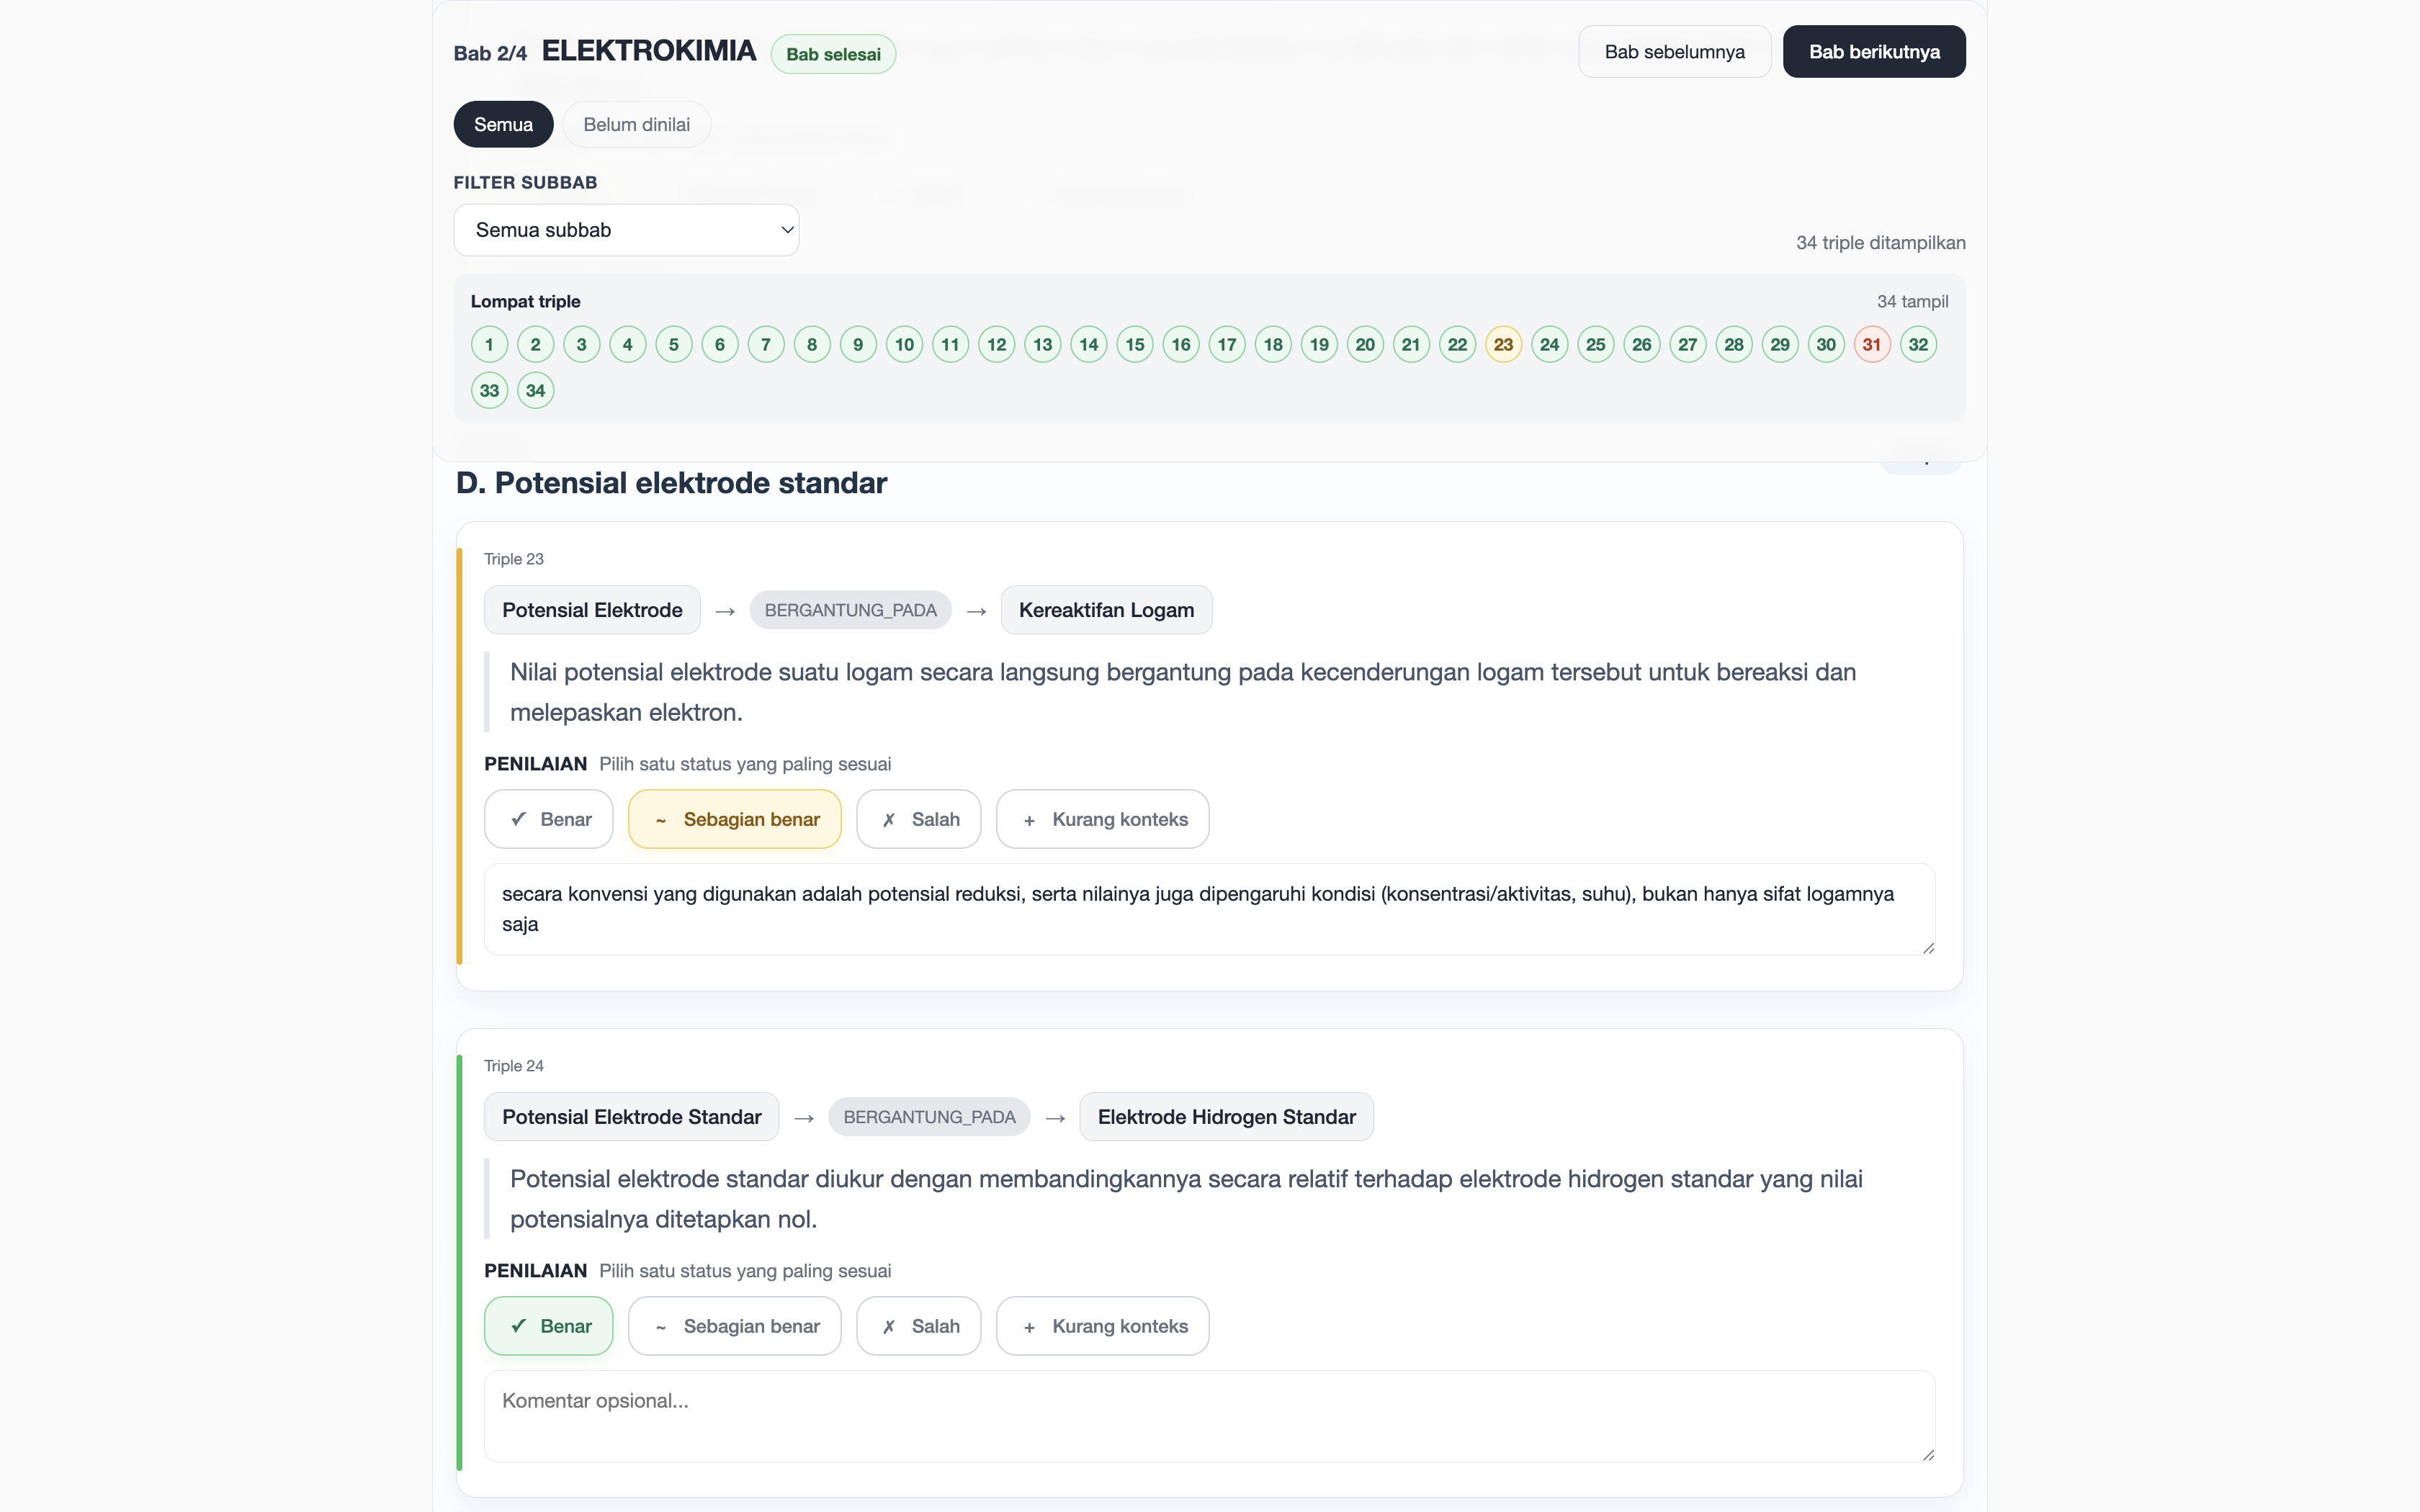
\includegraphics[width=\linewidth]{figures/phase1-interface.png}
  \caption{Antarmuka Fase~1: peninjauan \textit{triple} dalam-buku oleh pakar,
    dengan empat kategori penilaian (Benar, Sebagian benar, Salah, Kurang
    konteks) dan kolom komentar}
  \label{fig:review-app-phase1}
\end{figure}

\begin{figure}[h]
  \centering
  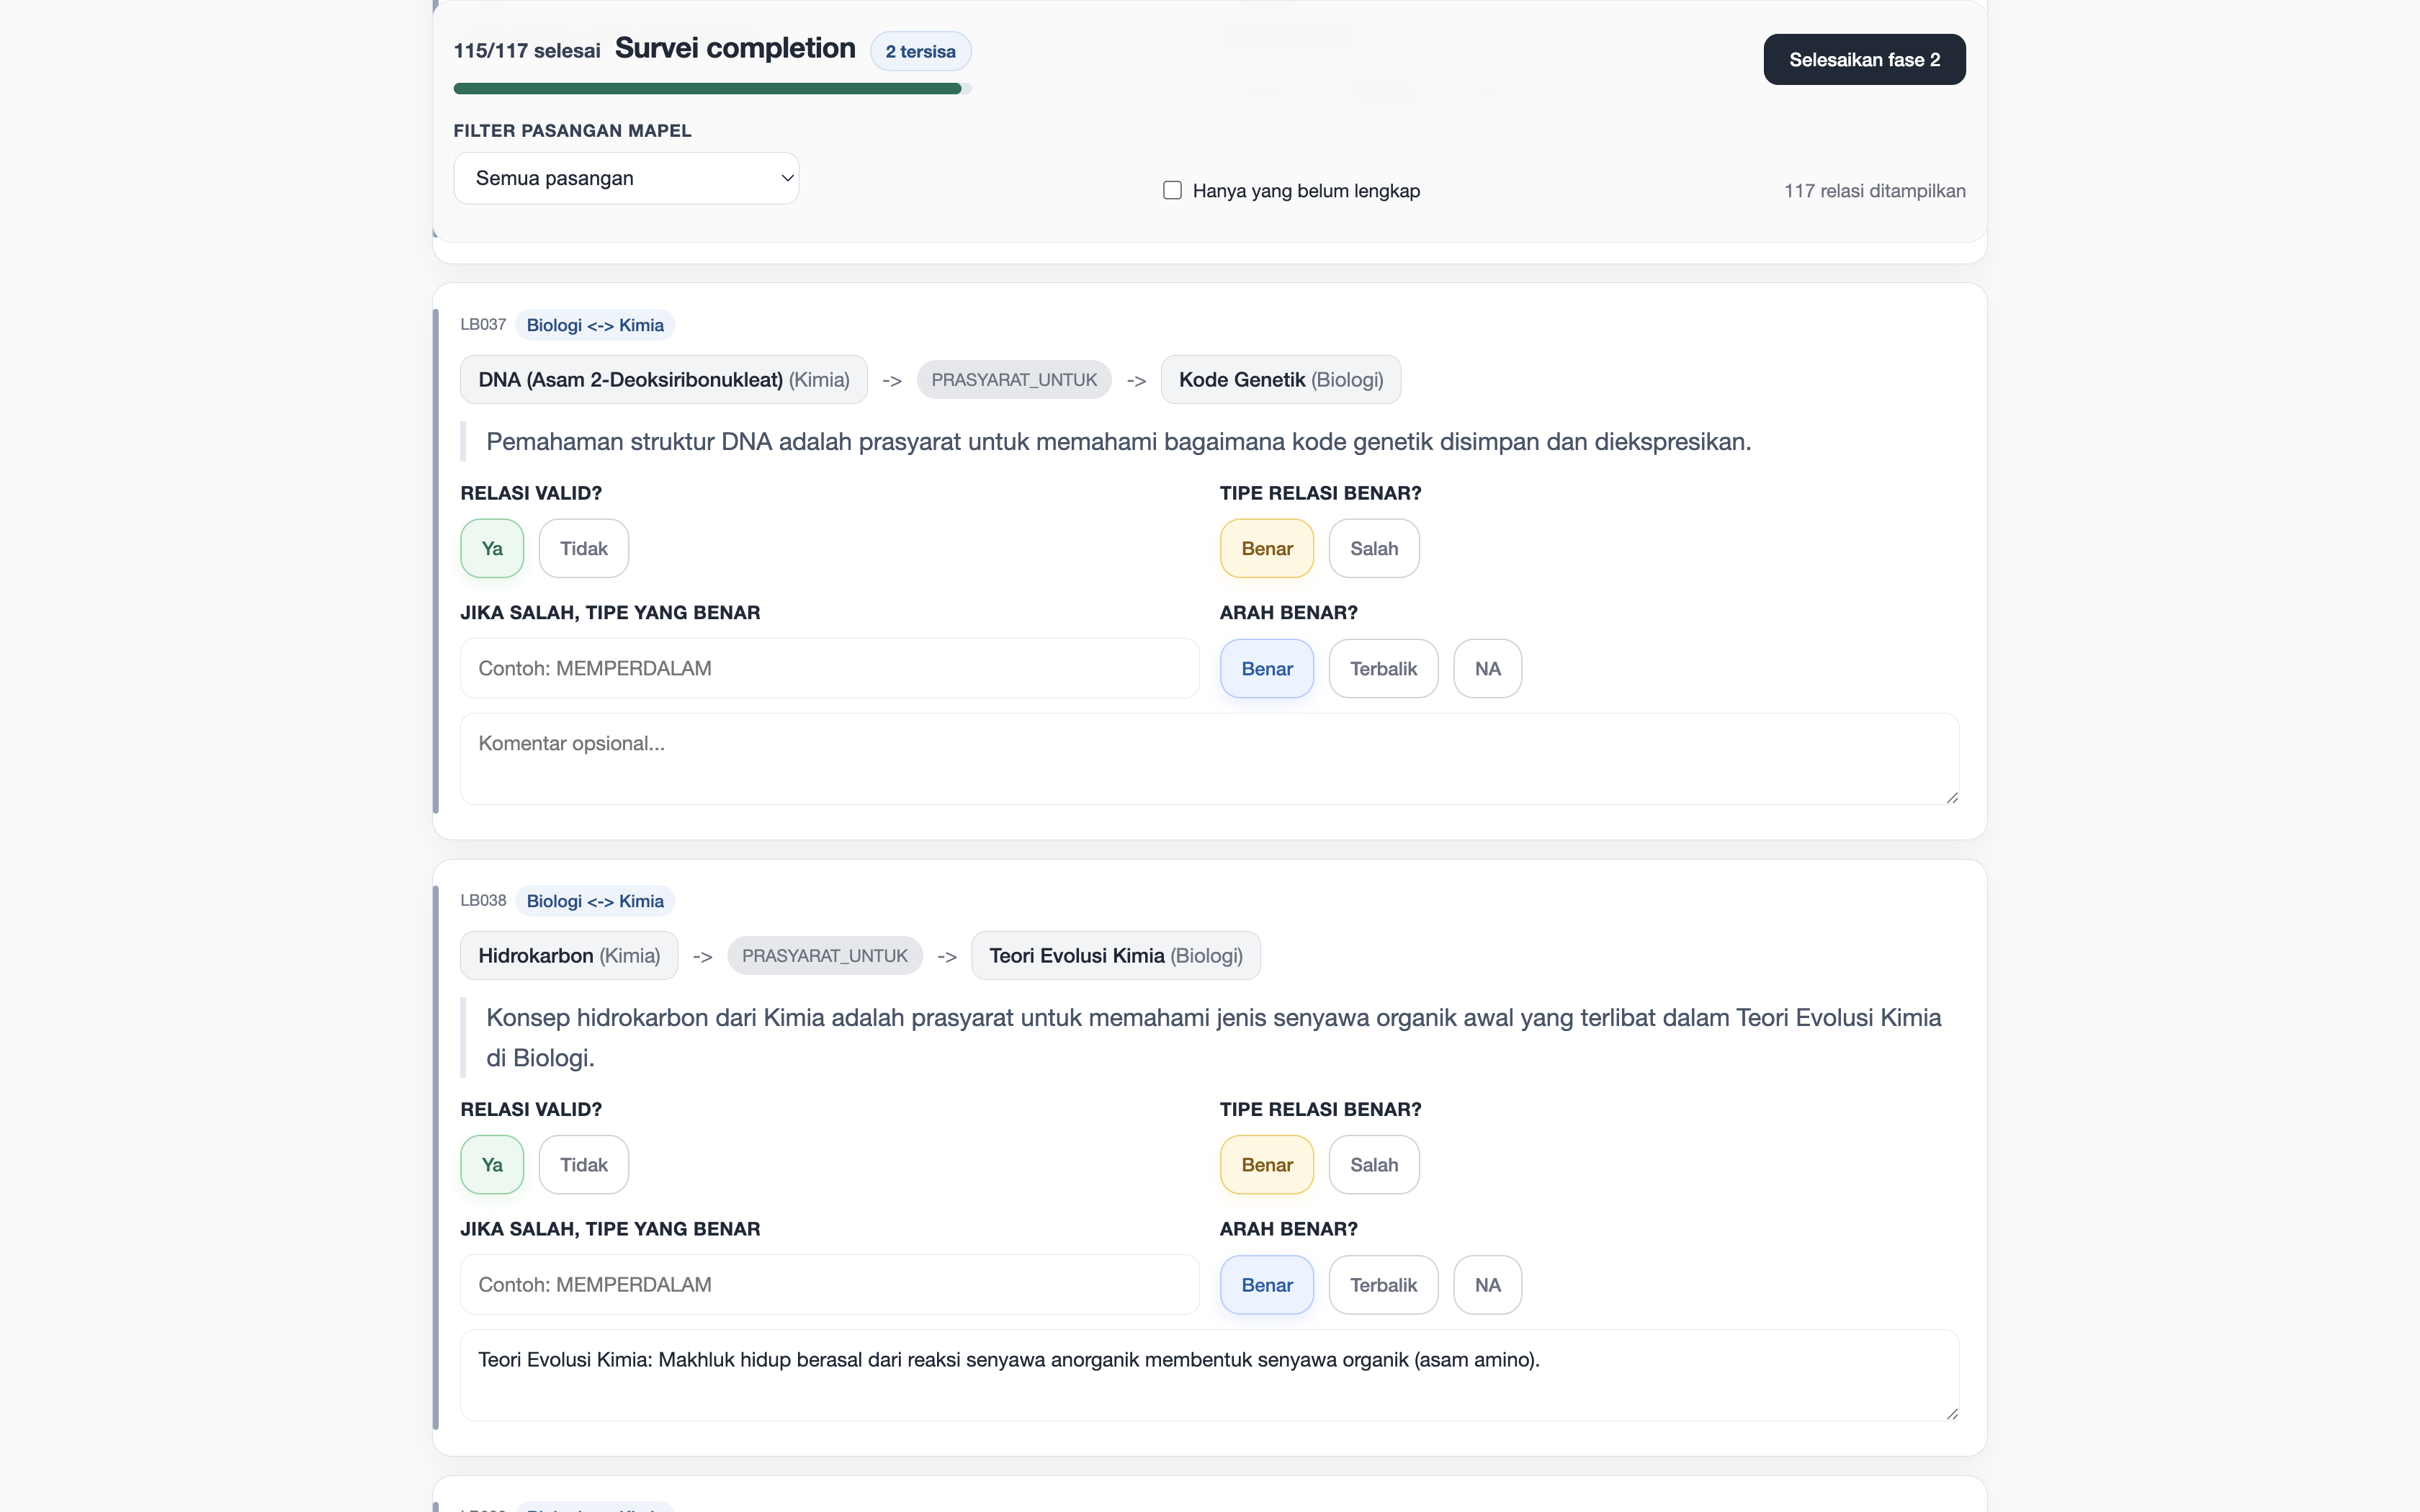
\includegraphics[width=\linewidth]{figures/phase2-interface.png}
  \caption{Antarmuka Fase~2: evaluasi diskusi \textit{edge} \textit{completion}
    lintas-buku, lengkap dengan kolom validitas relasi, ketepatan tipe, arah,
    dan komentar}
  \label{fig:review-app-phase2}
\end{figure}

\end{document}
